% Chapter 3

\chapter{Document Similarity} % Main chapter title

\label{Chapter 3} % For referencing the chapter elsewhere, use \ref{Chapter1} 

\lhead{Chapter 3. \emph{Document Similarity}} % This is for the header on each page - perhaps a shortened title

%----------------------------------------------------------------------------------------

\section{Lexical Similarity}
Similarity Measures for Text Document Clustering
                  Anna Huang
       Department of Computer Science
The University of Waikato, Hamilton, New Zealand
             lh92@waikato.ac.nz\\

In linguistics, lexical similarity is a measure of the degree to which the word sets of two given languages  are similar. A lexical similarity of 1 (or 100\%) would mean a total overlap between vocabularies, whereas 0 means there are no common words. (wiki)\\


\subsection{Document Represenatation}
There are several ways to model a text document. For example, it can be represented as a bag of words, where words are assumed to appear independently and the order is immaterial. The bag of word model is widely used in information retrieval and text mining [21]. Words are counted in the bag, which differs from the mathematical definition of set. Each word corresponds to a dimension in the resulting data space and each document then becomes a  vector consisting of non-negative values on each dimension. Here we use the frequency of each term as its weight, which means terms that appear more frequently are more important and descriptive for the document.
Let D = $\{d_1 , . . . , d_n \}$ be a set of documents and T = $\{t_1 , . . . ,t_m \}$ the set of distinct terms occurring in D. We discuss more precisely what we mean by "terms" below: for the moment just assume they are words. A document is then represented as a m-dimensional vector $t_d$.\\
Let tf (d, t) denote the frequency of term $t \,\epsilon\, T$ in document $d \, \epsilon\, D$. Then the vector representation of a document d is
\begin{equation}
\vec{t_{a}} = (tf(d,t_1,.....,tf(d,t_m))
\end{equation}
Although more frequent words are assumed to be more important as mentioned above, this is not usually the case in practice. For example, words like a and the are probably the most frequent words that appear in English text, but neither are descriptive nor important for the document’s subject.
\begin{figure}[htbp]
	\centering
		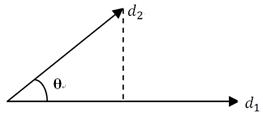
\includegraphics{./Figures/a.png}
		\rule{35em}{0.5pt}
	\caption[Angle Between Documents]{Angle Between Documents}
	\label{fig:Angle Between Documents}
\end{figure}
In fact, more complicated strategies such as the tfidf weighting scheme as described below is normally used instead.
With documents presented as vectors, we measure the degree of similarity of two documents as the correlation between their corresponding vectors, which can be further quantified as the cosine of the angle between the two vectors.
Figure 1 shows the angle in two-dimensional space but in practice the document space usually has tens and thousands of dimensions. Some useful properties of the cosine measure are discussed in Section 3.3.
\subsection{Similarity Measures}
\subsubsection{Eculidean Distance}
Euclidean distance is a standard metric for geometrical problems. It is the ordinary distance between two points and can be easily measured with a ruler in two- or three-dimensional space. Euclidean distance is widely used in clustering problems, including clustering text. It satisfies all the above four conditions and therefore is a true metric. It is also the default distance measure used with the K-means algorithm.\\
Measuring distance between text documents, given two documents $d_{a} and  d_{b}$ represented by their term vectors  $\overrightarrow{t_{a}} \,and\, \overrightarrow{t_{b}}$ respectively, the Euclidean distance of the two documents is defined as
where the term set is T = {t1 , . . . , tm }. As mentioned previously, we use the tf idf value as term weights, that is
crucial for cluster analysis, especially for a particular type w_{t,a} = tf idf (d_{a} , t).


\subsubsection{Cosine Similarity}
\When documents are represented as term vectors, the similarity of two documents corresponds to the correlation between the vectors. This is quantified as the cosine of the angle between vectors, that is, the so-called cosine similarity. Cosine similarity is one of the most popular similarity measure applied to text documents, such as in numerous information retrieval applications [21] and clustering too [9].
Given two documents $\overrightarrow{t_{a}} \,and\, \overrightarrow{t_{b}}$, their cosine similarity is

\begin{equation}
SIM_{c}(\vec{t_{a}},\vec{t_{b}}) =\frac{\vec{t_{a}}.\vec{t_{b}}}{|\vec{t_{a}}|\times|\vec{t_{b}}|}
\end{equation}

where $\overrightarrow{t_{a}} \,and\, \overrightarrow{t_{b}}$ are m-dimensional vectors over the term set T = \{t1 , . . . , tm \}. Each dimension represents a term with its weight in the document, which is non-negative. As a result, the cosine similarity is non-negative and bounded between [0,1].
An important property of the cosine similarity is its independence of document length. For example, combining two identical copies of a document d to get a new pseudo document d , the cosine similarity between d and d is 1, which means that these two documents are regarded to be identical. Meanwhile, given another document l, d and d will



%----------------------------------------------------------------------------------------

\section{Semantic Similarity}
            Corpus-based and Knowledge-based Measures
                           of Text Semantic Similarity
Rada Mihalcea and Courtney Corley                      Carlo Strapparava
     Department of Computer Science       Istituto per la Ricerca Scientifica e Tecnologica
        University of North Texas                              ITC – irst
        {rada,corley}@cs.unt.edu                            strappa@itc.it


Measures of semantic similarity have been traditionally defined between words or concepts, and much less between text segments consisting of two or more words. The emphasis on word-to-word similarity metrics is probably due to the availability of resources that specifically encode relations between words or concepts (e.g. WordNet), and the various testbeds that allow for their evaluation (e.g. TOEFL or SAT analogy/synonymy tests). Moreover, the derivation of a text-to-text measure of similarity starting with a word based semantic similarity metric may not be straightforward,and consequently most of the work in this area has considered mainly applications of the traditional vectorial model,occasionally extended to n-gram language models.
Given two input text segments, we want to automatically derive a score that indicates their similarity at semantic level,thus going beyond the simple lexical matching methods traditionally used for this task. Although we acknowledge the fact that a comprehensive metric of text semantic similarity  should also take into account the structure of the text, we take a first rough cut at this problem and attempt to model the semantic similarity of texts as a function of the semantic similarity of the component words. We do this by combining metrics of word-to-word similarity and word specificity into a formula that is a potentially good indicator of the semantic similarity of the two input texts.\\
   The following section provides details on eight different corpus-based and knowledge-based measures of word semantic similarity. In addition to the similarity of words, we also take into account the specificity of words, so that we can give a higher weight to a semantic matching identified between two specific words (e.g. collie and sheepdog), and give less importance to the similarity measured between generic concepts (e.g. get and become). While the specificity of words is already measured to some extent by their depth in the semantic hierarchy, we are reinforcing this factor with a corpus-based measure of word specificity, based on distributional information learned from large corpora.The specificity of a word is determined using the inverse document frequency (idf) introduced by Sparck-Jones (1972), defined as the total number of documents in the corpus divided by the total number of documents including that word. The idf measure was selected based on previous work that theoretically proved the effectiveness of this weighting approach (Papineni 2001). In the experiments reported here, document frequency counts are derived starting with the British National Corpus – a 100 million words corpus of modern English including both spoken and written genres.\\
   Given a metric for word-to-word similarity and a measure of word specificity, we define the semantic similarity of two text segments T1 and T2 using a metric that combines the semantic similarities of each text segment in turn with respect to the other text segment. First, for each word w in the segment T1 we try to identify the word in the segment T2 that has the highest semantic similarity (maxSim(w, T2 )), according to one of the word-to-word similarity measures described in the following section. Next, the same process is applied to determine the most similar word in T1 starting with words in T2 . The word similarities are then weighted with the corresponding word specificity, summed up, and normalized with the length of each text segment. Finally the resulting similarity scores are combined using a simple average. Note that only open-class words and cardinals can participate in this semantic matching process. As done in previous work on text similarity using vector-based models, all function words are discarded.
    The similarity between the input text segments $T_1 and T_2$ is therefore determined using the following scoring function:
    
\begin{equation}
SIM({T_{1}},{T_{2}}) =\frac{1}{2}(\frac{\sum_{w\in \{T_1\}} (maxSim(w,T_2 * idf(w)))}{\sum_{w\in \{T_1\}} idf(w)} + \frac{\sum_{w\in \{T_2\}} (maxSim(w,T_1 * idf(w)))}{\sum_{w\in \{T_2\}} idf(w)})
\end{equation}

   This similarity score has a value between 0 and 1, with a score of 1 indicating identical text segments, and a score of 0 indicating no semantic overlap between the two segments.Note that the maximum similarity is sought only within classes of words with the same part-of-speech. The rea-
son behind this decision is that most of the word-to-word knowledge-based measures cannot be applied across parts-of-speech, and consequently, for the purpose of consistency,we imposed the “same word-class” restriction to all the word-to-word similarity measures. This means that, for instance, the most similar word to the noun flower within the text “There are many green plants next to the house” will be sought among the nouns plant and house, and will ignore the words with a different part-of-speech (be, green, next). Moreover, for those parts-of-speech for which a word-to-word semantic similarity cannot be measured (e.g. some knowledge-based measures are not defined among adjectives or adverbs), we use instead a lexical match measure,
which assigns a maxSim of 1 for identical occurrences of a word in the two text segments.


\subsection{Corpus Based}

This \LaTeX{} Thesis Template is originally based and created around a \LaTeX{} style file created by Steve R.\ Gunn from the University of Southampton (UK), department of Electronics and Computer Science. You can find his original thesis style file at his site, here:\\
\href{http://www.ecs.soton.ac.uk/~srg/softwaretools/document/templates/}{\texttt{http://www.ecs.soton.ac.uk/$\sim$srg/softwaretools/document/templates/}}

My thesis originally used the `\texttt{ecsthesis.cls}' from his list of styles. However, I knew \LaTeX{} could still format better. To get the look I wanted, I modified his style and also created a skeleton framework and folder structure to place the thesis files in.

This Thesis Template consists of that modified style, the framework and the folder structure. All the work that has gone into the preparation and groundwork means that all you have to bother about is the writing.

Before you begin using this template you should ensure that its style complies with the thesis style guidelines imposed by your institution. In most cases this template style and layout will be suitable. If it is not, it may only require a small change to bring the template in line with your institution's recommendations.


\subsection{Knowledge Based}
Evaluating semantic relatedness using network representations is a problem with a long history in arti cial intelligence and psychology, dating back to the spreading activation approach of Quillian (1968) and Collins and Loftus (1975). Semantic similarity represents a special case of semantic relatedness: for example, cars and gasoline would seem to be more closely related than, say, cars and bicycles, but the latter pair are certainly more similar.\\
Rada et al. (Rada, Mili, Bicknell, & Blettner, 1989) suggest that the assessment of similarity in semantic networks can in fact be thought of as involving just taxonomic (is-a) links, to the exclusion of other link types; that view will also be taken here, although admittedly links such as part-of can also be viewed as attributes that contribute to similarity (cf.Richardson, Smeaton, & Murphy, 1994; Sussna, 1993).\\

Although many measures of similarity are de ned in the literature, they are seldom accompanied by an independent characterization of the phenomenon they are measuring, particularly when the measure is proposed in service of a computational application (e.g.,similarity of documents in information retrieval, similarity of cases in case-based reasoning).\\
Rather, the worth of a similarity measure is in its utility for the given task. In the cognitive domain, similarity is treated as a property characterized by human perception and intuition,in much the same way as notions like \plausibility" and \typicality." As such, the worth of a similarity measure is in its delity to human behavior, as measured by predictions of human performance on experimental tasks. The latter view underlies the work in this article, although the results presented comprise not only direct comparison with human performance but also practical application to problems in natural language processing.\\
    A natural, time-honored way to evaluate semantic similarity in a taxonomy is to measure the distance between the nodes corresponding to the items being compared | the shorter the path from one node to another, the more similar they are. Given multiple paths, one
takes the length of the shortest one (Lee, Kim, & Lee, 1993; Rada & Bicknell, 1989; Rada et al., 1989).\\
    A widely acknowledged problem with this approach, however, is that it relies on the notion that links in the taxonomy represent uniform distances. Unfortunately, uniform link distance is di cult to de ne, much less to control. In real taxonomies, there is wide
variability in the \distance" covered by a single taxonomic link, particularly when certain sub-taxonomies (e.g., biological categories) are much denser than others. For example, in WordNet (Miller, 1990; Fellbaum, 1998), a widely used, broad-coverage semantic network for English, it is not at all di cult to nd links that cover an intuitively narrow distance (rabbit ears is-a television antenna) or an intuitively wide one (phytoplankton
is-a living thing). The same kinds of examples can be found in the Collins COBUILD Dictionary (Sinclair, ed., 1987), which identi es superordinate terms for many words (e.g.,safety valve is-a valve seems much narrower than knitting machine is-a machine).\\
    In the rst part of this article, I describe an alternative way to evaluate semantic similarity in a taxonomy, based on the notion of information content. Like the edge-counting method, it is conceptually quite simple. However, it is not sensitive to the problem of varying link distances. In addition, by combining a taxonomic structure with empirical probability estimates, it provides a way of adapting a static knowledge structure to mul-
tiple contexts. Section 2 sets up the probabilistic framework and de nes the measure of semantic similarity in information-theoretic terms, and Section 3 presents an evaluation of the similarity measure against human similarity judgments, using the simple edge-counting method as a baseline.
    In the second part of the article, Sections 4 and 5, I describe two applications of semantic similarity to problems of ambiguity in natural language. The rst concerns a particular case of syntactic ambiguity that involves both coordination and nominal compounds, each of which is a pernicious source of structural ambiguity in English. Consider the phrase food handling and storage procedures: does it represent a conjunction of food handling and storage procedures, or does it refer to the handling and storage of food? The second application concerns the resolution of word sense ambiguity | not for words in running text, which is a large open problem (though cf. Wilks & Stevenson, 1996), but for groups of related words
as are often discovered by distributional analysis of text corpora or found in dictionaries and thesauri. Finally, Section 6 discusses related work.
\subsubsection{Wu \& Palmer}
    If words can be defined with concepts in a hierarchical structure, it is possible to measure the meaning similarity between words with an information measure based on WordNet (Resnik,1993), or structure level information based on a thesaurus (Kurohashi and Nagao, 1992). How-
ever, verb meanings are difficult to organize in a hierarchical structure.\\
In each conceptual domain, lexicalized concepts can be organized in a hierarchical structure. Within one conceptual domain, the similarity of two concepts is defined by how closely they are related in the hierarchy, i.e., their structural relations.\\

The Wu and Palmer (Wu & Palmer 1994) similarity metric measures the depth of two given concepts in the WordNet taxonomy, and the depth of the least common subsumer (LCS), and combines these figures into a similarity score:

\begin{equation}
SIM({T_{1}},{T_{2}}) =\frac{2 * depth(LCS)}{depth(concept_1)+ depth(concept_2)} 
\end{equation}

REfer: VERB SEMANTICS AND LEXICAL  SELECTION,Zhibiao Wu Martha Palmer


\subsection{Weigthing Factor}
\subsubsection {Specificity}
The following section provides more insight into term Specificity, which is the idea that some words carry more semantic content than others which is also referred to as Semantic Informativeness. Computational estimation of this quantity, term specificity, is important for various applications such as information retrieval. Here in addition to the similarity of words, we also take into account the specificity of words, so that we can give a higher weight to a semantic matching identified between two specific words (e.g. collie and sheepdog), and give less importance to the similarity measured between generic concepts (e.g. get and become). While the specificity of words is already measured to some extent by their depth in the semantic hierarchy, we are reinforcing this factor with a corpus-based measure of word specificity, based on distributional information learned from large corpora.
We use two methods of computing term specificity. The first method based on modeling the rate of learning of word meaning in Latent Semantic Analysis (LSA), LSA-Specificity. The second method is TF/IDF-Specificity.

\subsubsection{Latent Semantic Analysis – Specificity:}
In the following section we explain using Latent Semantic Analysis for approximating term Informativeness. Latent Semantic Analysis (LSA) is a language model that represents semantic word meaning as vectors in high-dimensional space. Word vectors are positioned in such a way that semantically-related words vectors point in similar directions or have a smaller angle / higher cosine between them. The representation is derived in an unsupervised manner, by observing occurrence patterns of words in a large corpus of natural language documents. Singular Value Decomposition (SVD) on the matrix of word/document occurrence counts is used to derive the optimal set of dimensions of the space in which all of the words can be represented as vectors. The number of dimensions is then artificially reduced to a smaller number (typically around 300) of most important dimensions, which has the effect of smoothing out incidental relationships and preserving significant ones between words. The resulting geometric space allows for straightforward representation of meaning of words and/or documents; the latter are simply a weighted geometric composition of constituent word vectors. Similarity in meaning between a pair of words or documents can be obtained by computing the cosine between their corresponding vectors. For details of LSA, please see (Landauer et al., 2007), and others.\\
LSA applications almost always focus on computing the semantic similarity between words (terms). However, another property of LSA, that has a significant effect, is the term vector length. The vector length plays a very important role in many LSA calculations, in particular – in giving relative weights to the word vectors that constitute a particular text passage. As (Kintsch, 2001) wrote, “Intuitively, the vector length tells us how much information LSA has about this vector. [...] Words that LSA knows a lot about (because they appear frequently in the training corpus [...]) have greater vector lengths than words LSA does not know well. Function words that are used frequently in many different contexts have low vector lengths -- LSA knows nothing about them and cannot tell them apart since they appear in all contexts”.
The metric of term Informativeness, or specificity, which we call LSAspec, is simply the ratio of LSA word vector length to the number of documents in the LSA training corpus that contain a particular word;
Missing Equation\\
Paper section 3.3\\
The value can be interpreted as the rate of vector length growth. We argue that more specific, or informative, words have the greatest rate of vector length growth; LSA learns about their meaning faster, with relatively fewer exposures. To illustrate this concept, let's look at a few examples that were obtained by controlling the number of occurrences of a particular word in the LSA training corpus. \\
@Mohsen: Should provide a graph for the relation of Vector lengths for some words vs. the number of documents containing those words.\\

\subsubsection{Inverse Document Frequency – Specificity:}
The specificity of a word is determined using the inverse document frequency (IDF) introduced by (Sparck-Jones, 1972), defined as the total number of documents in the corpus divided by the total number of documents including that word. The IDF measure was selected based on previous work that theoretically proved the effectiveness of this weighting approach (Papineni, 2001). Sparck Jones (1973) defines IDF as the probability of occurrence of documents containing a particular word.\\
IDF equation and definition of its terms\\
Where D is the total number of documents in the corpus. The assumption behind it is that low frequency words tend to be rich in content, and vice versa.
The term count in the given document is simply the number of times a given term appears in that document. This count is usually normalized to prevent a bias towards longer documents (which may have a higher term count regardless of the actual importance of that term in the document) to give a measure of the importance of the term t within the particular document d. One well-studied technique is to normalize the TF weights of all terms occurring in a document by the maximum TF in that document.\\
http://nlp.stanford.edu/IR-book/html/htmledition/maximum-tf-normalization-1.html
%----------------------------------------------------------------------------------------
\subsection{Disambiguation}
\lstset{language=Pascal}          % Set your language (you can change the language for each code-block optionally)
 
\begin{lstlisting}[frame=single]                % Start your code-block
Input: Sequence W = {wi |i = 1..N }
Input: Admissible labels Lwi = {lwi |t = 1..Nwi },i = 1..N
Output: Sequence of labels L = {lwi |i = 1..N }, with label lwi corresponding to word wi from the input sequence.
Build graph G of label dependencies
1: for i = 1 to N do
2: for j = i + 1 to N do
3: if j − i > M axDist then
4: break
5:end if
6:for t = 1 to Nwi do
7:for s = 1 to Nwj do
8:weight ← Dependency(lwi , lwj , wi , wj )
9:if weight > 0 then
10:AddEdge(G, lwi , lwj , weight)
11:end if
12:            end for
13:        end for
14:    end for
15: end for
Score vertices in G
1: for all Va ∈ V ertices(G) do
2: Score(Va ) ← Centrality(Va )
3: end for
Label assignment
1: for i = 1 to N do word.                                                                                                 t
2: lwi ← argmax{W P (lwi )|t = 1..Nwi }
3: end for
\end{lstlisting}
\subsection{ay7aga}
